% TEMPLATE for Usenix papers, specifically to meet requirements of
%  USENIX '05
% originally a template for producing IEEE-format articles using LaTeX.
%   written by Matthew Ward, CS Department, Worcester Polytechnic Institute.
% adapted by David Beazley for his excellent SWIG paper in Proceedings,
%   Tcl 96
% turned into a smartass generic template by De Clarke, with thanks to
%   both the above pioneers
% use at your own risk.  Complaints to /dev/null.
% make it two column with no page numbering, default is 10 point

% Munged by Fred Douglis <douglis@research.att.com> 10/97 to separate
% the .sty file from the LaTeX source template, so that people can
% more easily include the .sty file into an existing document.  Also
% changed to more closely follow the style guidelines as represented
% by the Word sample file. 

% Note that since 2010, USENIX does not require endnotes. If you want
% foot of page notes, don't include the endnotes package in the 
% usepackage command, below.

\documentclass[letterpaper,twocolumn,10pt]{article}
\usepackage{usenix,epsfig,endnotes}
\begin{document}

%don't want date printed
\date{}

%make title bold and 14 pt font (Latex default is non-bold, 16 pt)
\title{\Large \bf Saving pins and power with integrated voltage converters}

\author{
{\rm Michael Barrow}\\
mbarrow@eng.ucsd.edu\\
University of California, San Diego
%\and
%{\rm Second Name}\\
%Second Institution
}

\maketitle

% Use the following at camera-ready time to suppress page numbers.
% Comment it out when you first submit the paper for review.
\thispagestyle{empty}


\subsection*{Abstract}
Recently, demand for increased processor performance coupled with reducing power budget has been addressed using emerging parallel processors. Parallel computation is an energy efficient \textbf{(cite chandrakasan)} way of increasing performance but requires wider interconnect busses. At the die boundary, the consequence is that systems face an IO bottleneck. The connection between silicon and substrate ends the scope of Moores law in a system, with IO density of packages increasing at a slower rate than on chip.\\
Compounding this problem, addressing performance by increasing paralell units result in increasing energy density due to the end of Dennard scaling \textbf{(cite)}. Devices therefore require an increasing number of power pins, further limiting IO pin availability. \textbf{HOW ABOUT COMPELLING EXAMPLE?}
We examine integrated power converters in this context. A review of the literature suggests with further research this technique could address the IO bottleneck of future processors.% and power efficiency of future processors.         

\section{Introduction}

%As Moores law continues, Technology scaling gives an increasing number of building blocks to meet conflicting consumer demands of increasing performance and energy efficiency. However the turn right approach exposes architects to complications of inconsistent technology scaling rates. In particular, for IO bound applications, the amount of achievable parallelism in silicon is proportional to the number of IO pins. The  \\

%\begin{itemize}
%\item{\textbf{Motivation}:  crisis has been known for some ti}
%\item{Stakeholders}
%\item{Historical context}
%\item{Current state of art}
%\item{State of art limitations}
%\item{Content of doc}
%\end{itemize}

Against a backdrop of declining PC and growing smartphone sales, mobile devices drive demand for low power, high performance architectures. Emerging applications such as augmented reality, location aware services, high performance games and novel machine interfaces place an increasing demand for expanded IO capabilities and memory bandwidth from generation to generation of these devices. With the number of popular software stacks being lower than the number of major hardware vendors, device battery life is an important product differentiator. Research interest has therefore increased in power efficient architectures that can meet the IO and memory bandwidth requirements of the mobile segment.\\
%DROP THISDespite a drop in PC demand, server 
\indent package IO density is a well known problem to architects. Marbell et al~\cite{Marbell2011} review 130 hardware designs over 30 years and conclude the historical trend of package pin count and power pin count increase at an unsustainable rate. Promising solutions have been proposed, with Chang et al~\cite{Chang2010} identifying a subset of practical approaches in 2010. They conclude that voltage scaling as proposed by Dennard et al~\cite{Dennard1974} is feasible, but enabled by a sum of techniques in different disciplines.\\
At the architectural level, power converter integration is advised in the worst case, where challenges of sub-threshold leakage prevent further reduction of CMOS voltage and power density prevents further integration of IO intensive system blocks such as memory. The observation in~\cite{Chang2010} is that reducing CMOS voltage has an exponential impact on loss through the power delivery pins. By maintaining pin voltage to devices and reducing operating voltage of CMOS using an efficient on die DC DC voltage converter bridge, an IC has a higher effective power density without increasing the number of power pins.\\
\indent Research into integrated DC DC converters has been an active topic pre-empting~\cite{Chang2010} for other architectural benefits. As will be seen in detail in section \textbf{SECTION No}, DC DC converters typically feature bulky passive components. These increase the cost and footprint of mobile systems. Additionally, battery technology does not enjoy the improvement rate of CMOS, so operating voltage drops have opened a gulf between Battery supply voltage and IC input voltages. Techniques for extending battery life such as multiple voltage domains mean CPU's require multiple supply voltages. The symptoms of this are seen in the \textbf{Quallcomm snapdraggon 800 which features 9 off chip DC DC converters CITE}. Against this backdrop, the feasibility of integrated DC DC converters shown by Kurson et al~\cite{Kurson2003} invigorated research interest of integrated DC DC converters. A major motivation is removing the space and component costs of off chip converters \textbf{CITE A bunch of papers that feature this in abstracts}.\\
\indent State of the art in integrated DC DC converters is exemplified in Intel Haswell CPU's FIVR. Although a comparable DC DC converter exists in the literature~\cite{Sturcken2012}, to the authors knowledge this is the only example of an integrated DC DC converter supplying a general purpose CPU in such a power envelope.\\
Intel's literature~\cite{Intel2010} %http://www.psma.com/sites/default/files/uploads/tech-forums-nanotechnology/resources/400a-fully-integrated-silicon-voltage-regulator.pdf
suggests the FVIR is employed primarily to remove external DC DC converters and improve power efficiency. However a comparison of the pinout between Haswell \textbf{Cite} and the non FIVR predecessor \textbf{Ivybridge Cite} suggests that some power pins were saved too. This is unsurprising as Kurson notes in~\cite{Kurson2003} that power pins could be saved by integrated DC DC converters. As we note DC DC converters improve the IO density problem, we review the literature to asses the feasibility of optimizing power pins to IO pins by increasing supply voltage of an integrated DC DC converter greatly beyond typical CPU operating voltage.\\
\indent The rest of the document is ordered as follows:\\
\begin{itemize}
\item{The operation of the DC DC converter and its critical design parameters}
\item{Challenges associated with integrating DC DC Converters on die}
\item{Performance limitations of monolithic CMOS DC DC converters}
\item{Summary of recent research in integrated DC DC converters}
\item{Methods of optimizing IC pin out with integrated DC DC converters}
\item{Conclusions}
\end{itemize}
 

%More fascinating text. Features\endnote{Remember to use endnotes, not footnotes!} galore, plethora of promises.\\

\section{Operation of the DC DC converter}

\textbf{Definition of the problem}\\
Two popular stepdown converters in the literature are presented. A review of the literature highlights critical properties the topologies must feature in order to integrate either on chip.

\subsection{Switched Capacitor stepdown converter operating principle}
%For SC description you can see: https://docs.google.com/a/eng.ucsd.edu/document/d/18fPNSis3hjVwwXtvNOv4B4ni1we3ly9B9yZqkZxr0No/edit
Two types of DC DC step down converter are popular in the literature. Type 1 is the switched capacitor (SC) converter. a simplified canoical $\frac{1}{2}$ series-parallel step-down topology is shown in Figure ~\ref{SCTopology}.\\


\begin{figure}[here]
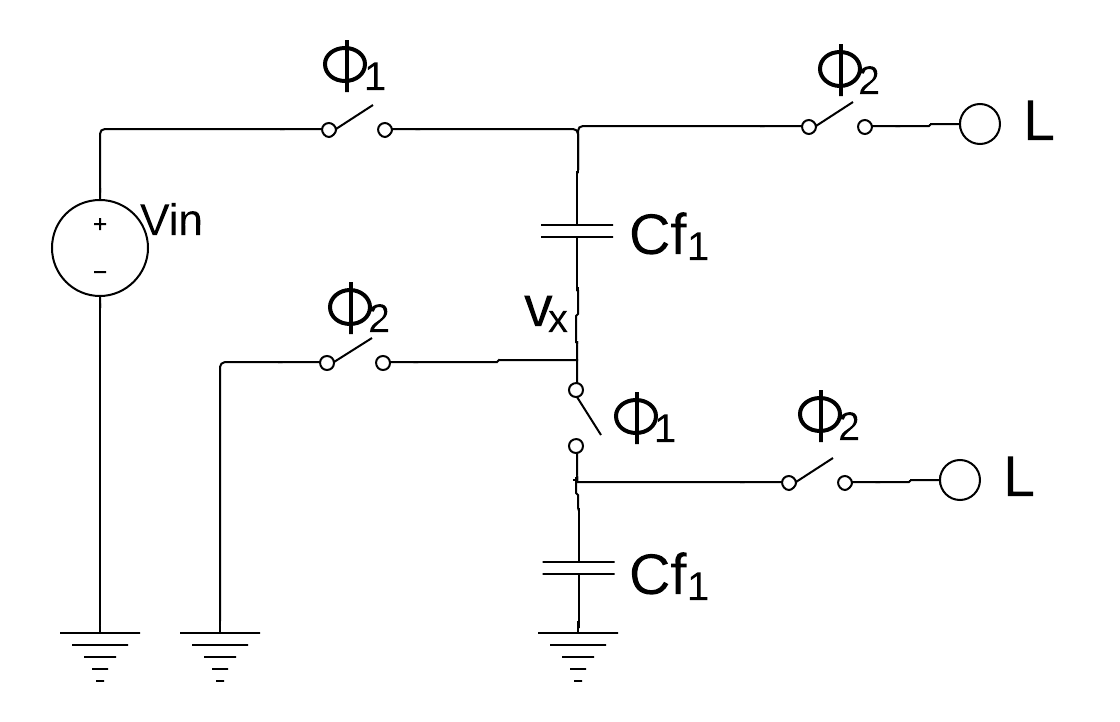
\includegraphics[width=0.4\textwidth]{SCTopology}
\caption{A $\frac{1}{2}$ stepdown SC topology}
\label{SCTopology}
\end{figure}

Let us consider the circuit with ideal components. $Cf$ denotes some capacitance such that $Cf_1 = Cf_2$. switches are controlled by mutually exclusive clocks, $\phi_1$ and $\phi_2$. These clocks are non-overlapping.\\
The circuit has two phases of operation. In phase 1, the charging phase, $\phi_1$ switches are closed and $\phi_2$ switches are open. $Cf_1$ and $Cf_2$ are in series. Since the capacitors are the same size, $V_x$ is $\frac{1}{2}$ of $V_in$.\\
In phase 2, the discharging phase, $\phi_2$ switches are closed and $\phi_1$ switches are open. Now $Cf_1$ and $Cf_2$ are in parallel. Since they are matched in size, $V_x$ remains at $\frac{1}{2}$ and is seen at terminal $L$ across both capacitors.\\

\subsection{Inductor-capacitor stepdown converter operating principle}

The second popular converter is the inductor-capacitor stepdown (buck) converter. A simplified canoical topology is shown in Figure~\ref{BKTopology}.\\
\begin{figure}[here]
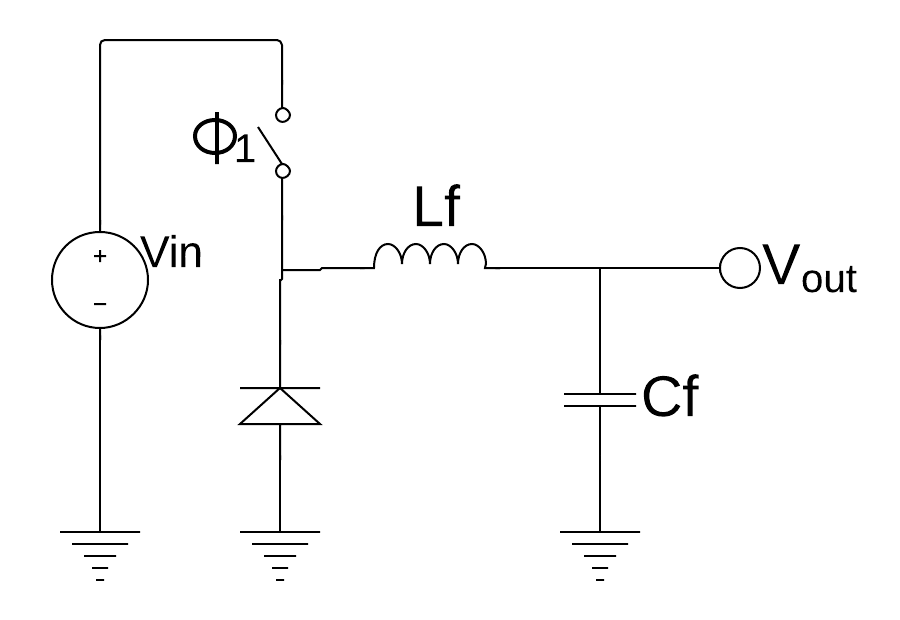
\includegraphics[width=0.4\textwidth]{BKTopology}
\caption{An inductor capacitor buck topology}
\label{BKTopology}
\end{figure}

%For Buck description use chapter 4 of Kurson
The voltage conversion principle is understood by considering the inductor and capacitor as a high pass filter. $\phi_1$ is a clock used to generate a square wave voltage of amplitude $V_{in}$. If this square wave is at a frequency sufficiently higher than the 3db cutoff frequency of the filter, only the DC component of the square wave is observed at $L$. Because of this, buck converters may change their voltage stepdown ratio during operation, by modulating $\phi_1$. For a properly designed converter, $V_L$ is defined by the duty cycle "$D$"~\cite{Kurson2006} of $\phi_1$ where: $V_{out} = V_{in} \times D$. In other words, if the square wave entering $L_f$ is high for $\frac{2}{3}$ of its period, $V_{out} = \frac{2}{3}\times V_{in}$ and $D = \frac{2}{3}$.\\ 

\subsection{SC stepdown converter critical parameters}
%Note the \textbf{introduction of $\phi_{\frac{2}{3}}$} This is introduced so when $Cf_2$ has discharged to the load, $Cf_1$ may be connected to restore the supply voltage seen at node $L$. \textbf{we do this because the parasitic resistance of $Cf_1$ and $Cf_2$ is larger in series, maintaining Vout for longer (also fucks with your load impedance, why do it??!!)}\textbf{WE SEE THAT IT IS CRITICAL TO HAVE HIGH FREQUENCY IN ORDER TO MAINTAIN SUPPLY VOLTAGE}
The energy that a SC converter can transfer per charge cycle is $E_{Isc} = CV^2$. We could therefore express $W = E_{Isc}\times F_\phi$.\\
$V$ For a design with a given $V_in$ and ideal components, the designer has two degrees of freedom to power a load, $C$ and $F_\phi$.\\  
We re-draw Figure~\ref{SCTopology} with non-ideal components in Figure~\ref{NonIdealSCTopology}.\\

By observation of Figure~\ref{NonIdealSCTopology} we see that $F_\phi$ and $C$ are critical parameters that must be optimised for minimum losses\\
Losses associated with switches are switching loss during the non-overlapping period of $\phi$, and conduction loss due to the equivilent series resistance (ESR) of switches.\\
Conduction loss reduces the supply voltage seen at the capacitors by a factor $\delta V_a$. Conduction loss is therefore sensitive to the stepdown ratio. Increasing the stepdown ratio increases the number of series switches between all capacitors during the charging phase. For example a ratio of $\frac{1}{3}$ has 2 series switches, one of $\frac{1}{4}$ has 3 series switches and so on.\\
Losses associated with capacitors are parasitic capacitance losses. A parasitic capacitance known as bottom plate capacitance exists between one plate of each capacitor and ground. The voltage of these parasitic capacitor is a virtual ground and reduces the supply voltage seen at the capacitors by $\delta V_b$. Their charge can leak to true ground but cannot reach a load. As they are smaller than useful capacitance, they are significantly charged and discharged on each cycle of the converter. Loss is therefore expressed as $W = E_{Pc} \times F_\phi$ where $E_{Pc} = 1.5\alpha CV^2$. Literature reports bottom plate capacitance to be up to 5\% of $C_{tot}$~\cite{Ramadass2007}. We also note that $F_\phi$ is adjustable at runtime and $C$ is not and that $I_{out} \propto C$~\cite{Damak2013} as well as $F_\phi$.\\
%Move load regulation to different sub section SC converters by topology have difficulty 
In SC converters then, careful design considering voltage specification and technology parameters optimises converters to their load. 

\subsection{Inductor-capacitor converter critical parameters}

How it works, critical parameters

\subsection{Converter load regulation concept}
Load regulation is matching output impedance "$Z_O$" of a power converter to a current load. Because $I= \frac{V}{Z_O}$ and maintaining $V$ for a processor is critical, converter output impedance must track quickly with the load condition to keep $V$ constant. The responsibility of tracking load and adjusting $Z_O$ belongs to control circuits. Block Diagrams are shown in figure~\ref{ControlCKBlockDiags}\\
Inductor-capacitor converters can reduce $Z_O$ by increasing conductance. This is done by increasing "$D$" in eqn\textbf{REF EQN}. Because the asymtote is impedance of the filter at $F_S$, $Z_O$ may also be increased by reducing $F_S$.~\cite{Alghamdi2012}.\\ %may want to change ref...
SC converters power loads capacitively. Because the capacitors supply a DC load in parallel, $Z_O$ cannot be lowered below $Z_C$ + $Z_{Sw}$ at the nominal $F_{Sw}$. Modulating $F_{Sw}$ can increase impedance in practice, because the capacitors can be purposely under-charged~\cite{Seeman2008}.\\
%Talk about tradeoffs? No I think put that in problems  

\section{Design of Integrated DC DC Converters}

Practical integrated converters are emerging and designed with different goals. A taxonomy of reviewed literature identifies two groupings:\\
\textbf{1: Power system replacement converters}. The goal is to remove external VRMs with an equaly performing integrated subsystem\\
\textbf{2: LDO replacement converters}. The goal is an incremental improvement of the Low-dropout (LDO) regulators that have long been integrated on chip~\ref{MaximLDO}.\\
These differing goals result in different design tradeoffs. We focus on group 1 because of an efficiency reason. To explain, consider the operating principle of an LDO. A transistor gate is biased in its linear conduction region and a fixed voltage is dropped from source to drain to give desired $V_{Out}$. Recall power transfer efficiency, $\eta = \frac{R_{Load}}{R_{Load} + R_{Source}}$. For an LDO, \textbf{(MAX)}[$\eta$] = 0.5. Using a comparable integrated converter to optimize power pins is intractable because around half the power budget is wasted as heat, clearly a sub-optimal design. As such, literature aiming at group 1 best aligns with our interest in pin count optimisation.\\  

\subsection{Motivation}
Switching converters such as the SC and buck can offer far higher efficient energy transfer than linear types. Theoretical efficiencies have been modeled at 96\%~\cite{Rodriguez2014} using state of the art devices. Integrated buck and SC implementations have been reported with 84\%~\cite{Cheng2013} and 93\%~\cite{Damak2013} efficiency respectively. Provided these power converters can drive the desired load of a processor, they could be used to obtain an optimum IO to power pin ratio for a processor. This would be done by increasing the input voltage to on die converters to reduce the number of supply pins until a desired number is reached.  

\subsection{Design challenges}
An Integrated DC DC converter is optimized through design tradeoffs that consider component non-idealities. Given that CPU designs have differing power envelopes and CMOS processes have unique electrical properties, researchers have explored the design space at multiple entry vectors.\\  

%\textbf{Definition of the system problem lives in}\\
%History of research\\
%System type 1(Switched capacitor AND HISTORY)\\
\indent \textbf{SC converters} The entry vector is an argument that A: Capacitance is easy to implement because MOSFET gate capacitance is a basic building block of CMOS. No corresponding basic block exists for inductance. B: Inductors have a necessarily large parasitic impedance because they are made from coiled resistive wire. Capacitors have a lower minimum impedance which shrinks as the plate size or capacitance grows.\\
However, as we have seen this type of converter has less flexible output impedance as compared with buck converters. Also SC converters do not have a voltage regulating filter which is built-in to bucks. This makes their output voltage vunerable to switching noise.\\
Therefore the design challenges emphasised in SC converters are: maximising effective capacitance, controlling output impedance and regulating output voltage.\\ 
%\textbf{Problems of bottom plate parasitic cap}. Bottom plate parasitic capacitance limits the attractiveness of SC designs. \\
%Problems of switching noise. These designs are noisier than Bucks, which have a filter by design\\
\indent \textbf{buck converters} The entry vector is an argument that C: Inductors can be implemented in standard CMOS. D: Inductor based buck has been a preferred design for (>100mW) applications over the past several decades ~\cite{Sanders2010}, why change now?
%System type 2(Integrated buck AND HISTORY Kurson book)\\
%Want to show how General CMOS components are made for this role and why they didn't work.\\

%MOVE THIS DOWN INTO THE NEXT SECTION
%In the case of both SC and buck, researchers faced setbacks from their initial vectors. We summarize these setbacks with reference to arguments \textbf{A},\textbf{B},\textbf{C} and \textbf{D}
%\begin{itemize}
%\item \textbf{A} CMOS MOSFET gate capacitance has large leakage and low energy density \textbf{CITE}
%\item \textbf{B} Parallel advances in device physics were applied to inductors, greatly improving inductance to impedance ratio \textbf{CITE}
%\item \textbf{C} CMOS implementations of inductors have low energy per area so were prohibitively area expensive \textbf{CITE}
%\item \textbf{D} Circuit design techniques alone cannot compensate for the quality of components realisable in standard CMOS \textbf{CITE} 
%\end{itemize}
%END MOVE DOWN

\subsection{Performance drawbacks of Baseline monolithic DC DC Converters}
An example of a CMOS integrated SC converter \cite{Viraj2007} and CMOS integrated buck converter \cite{Alimadadi2008} are taken as examples. These designs highlight the performance drawbacks of baseline CMOS for integrated converters and explain the present concentration of research interest in this field. These setbacks from the initial entry vectors of the SC and buck camps also explain the research and design approaches taken in more recent work. Although one process generation separates the designs, they are reasonably compared since the power components (capacitors, inductors and switches) consume almost all of the die in both designs.\\
\textbf{SC drawbacks} Naive Integrated SC converters have a low power density. \cite{Viraj2007} realize an on die capacitance of 1600pF with a converter power density of 1.7$mW/mm^2$. In comparison  the baseline buck \cite{Alimadadi2008} realize on die capacitance of 1.1nF with a power density of 20$mW/mm^2$.\\
The baseline SC converter also realizes much lower efficiency than expected in\cite{Viraj2007}. $80\%$ is predicted in the literature, but only $62\%$ is achieved due to unmoddled losses.\\
Only a single step-down voltage ratio is implemented, since the fixed SC circuit topology described earlier is used.\\
The performance of this design focussed researchers in areas to make SC integrated converters attractive in replacing off chip IC power converters. Broad categories and related research are listed below.\\
\begin{itemize}
\item \textbf{Energy density: }Device technology research to improve capacitor energy density
\item \textbf{Efficiency: }Technology, circuit topology and converter control research to reduce power leakage
\item \textbf{Flexibility: }Improve load regulation with SC power circuit topology and SC converter control research. In other words, provide flexible step-down ratio's. 
\end{itemize}
\textbf{buck drawbacks} Although power density is higher than the baseline SC, it is still too low for contemporary processors. The combined area of the converter and load must feature an power density higher than that dissipated in the load \textbf{GET A GOOD REF OF POWER FOR MOBILE CPU'S}\\
Naive Integrated buck converters have a low efficiency. \cite{Alimadadi2008} achieve a peak efficiency of $46\%$. Not only is this lower than the baseline SC \cite{Viraj2007}, its lower than an LDO ($50\%$).\\
Unlike the SC design, the baseline buck can implement a range of stepdown voltages in a basic topology. However the baseline has poor load regulation. At its lowest output voltage it has a $25\%$ efficiency in its most sophisticated operating mode. This drops to $13\%$ in its baseline mode.\\ 
As with the SC design, the issues in this and other early monolithic converters led researchers to focus on areas for improvement to make integrated buck converters suitable to replace discrete IC's. Again we summarise broad categories and related research below.
\begin{itemize}
\item \textbf{Energy density: }Device technology research to improve inductor energy density
\item \textbf{Efficiency: }Technology, buck circuit topology and buck converter control research to reduce power leakage
\item \textbf{Flexibility: }Improve load regulation with buck converter control research. Buck converter voltage stepdown was better understood than SC, but poorly controlled
\end{itemize}
The broad categories of buck overlap those of the SC researchers. Therefore some research effort may transfer between the two designs and we also observe a merge between the seperate research entry vectors identified earlier.\\
This manifests at the device level, where both converters share the same need to reduce losses. We can list these basic blocks and consider their problems when applied to integrated power converters abstractly from the two converter topologies.\\  
%\textbf{Taxonomy of problem (deeper drill and more specifics of the problem)}\\
%what is wrong with the switches?\\ %loss of sqrt(fs) A 10-MHz Green Mode Automatic... Cite THIS paper.
\textbf{CMOS Switches: }
Besides conduction losses, CMOS switches also suffer static and dynamic parasitic losses due to non-idealities. All must be balanced for an optimised power switch.\\ % In integrated 
\textbf{TRANSISTOR DIAGRAM SHOWING CRITICAL PARAMS}\\

Static losses are constant no matter if the MOSFET switch is on or off. They occur because the MOSFET does not have an infinite open circuit resistance. Static loss is therefore technology node dependent and impossible to remove completely. Static losses are contributed to by components from sub-threshold leakage and gate oxide leakage currents.\\
These losses are intrinsic to all transistor based switches, however tradeoffs possible in modern technology nodes for full integration are less optimal than older technologies. Aggressive technology scaling continuously increases transistor leakage\cite{Iwai2009}, so that realising the highest compute performance results in switches with the lowering efficiency in fully integrated designs.\\
Dynamic losses occur due to toggling the MOSFET switches. Power is consumed by changing the switch condition. As such, losses can be reduced by controlling switch toggling frequency, since for a given technology loss of the power switches and drivers increases by approximately $\sqrt{F_s}$\cite{Andreou1999}. However given fixed size energy transfer components, reducing $F_s$ reduces the converters power rating since $P = F_s \times E$.\\
Conduction loss occurs because the MOSFET switch does not have a zero on resistance. At a DC operating point, the conduction loss is simply the resistance of the MOSFET. Resistance of a MOSFET may be reduced by decreasing its channel length, $L_{ch}$ or increasing its channel width, $W_{ch}$. The minimum channel length is determined by process node e.g. $22_{nm}$ long in a $22_{nm}$ process, but channel width can be extended arbitrarily. However gate capacitance, $G_c \propto W_{ch} \times L_{ch}$. Reducing conduction loss therefore increases dynamic loss by increasing the power needed to charge $G_c$ and toggle the switch.\\  
\indent As a final note, CMOS switches cannot operate reliably beyond the technology node voltage. This imposes limitations on the stepdown voltage ratio that can be achieved if a switch is connected between power rails. This does not impact loss but it does mean that the power a converter can supply is maximum when the stepdown ratio is $1:1$ \textbf{TRUE KINDA BUT JUSTIfy WITH EQN}\\
\indent By considering a fully optimised switch, we see the pressing research problems are reversing the leakage trend\cite{Iwai2009} and operating with rail voltages above the target technology rating.\\ 
\textbf{Capacitors: }
Capacitors suffer from time or frequency related losses due to non-ideality. The loss problem is complicated by the frequency dependence of capacitor impedance/reactance. This is encapsulated with $Q_c=\frac{1}{\omega CR_c}$, or the capacitors "Q" quality factor. If $Q_c$ = 1, the capacitor is ideal and does not impede a voltage signal. The "Q" factor has a different level of criticality in SC and buck designs. buck designs can offset a low capacitor "$Q_c$" value with their inductor if properly designed.\\
\textbf{DIAGRAM SHOWING CRITICAL PARASITICS}\\
Because converters normally operate at a high frequency, Loss in the capacitor is typically due to its equivilant series resistance, $R_c$ and its parasitic capacitance. The major parasitic capacitance component is formed between the ground node and bottom plate of the capacitor\cite{Damak2013}. as noted previously CMOS may have up to 5\% parasitic capacitance. This is more critical for SC designs since they must transfer all of their energy via capacitors.\\
\indent Considering the loss mechanisms in a capacitor, improvements to integrated converters are not easily made at the architectural or circuit level. Important research questions involve critical technology parameters. We also observe buck converters are less sensitive to low quality capacitors.\\
\textbf{Inductors: }Inductors, similar to capacitors suffer from frequency related non-ideality as well as static DC loss. As such, they have a quality factor $Q_l = \frac{\omega L}{R_l}$. A $Q_l$ = 1 represents a perfect inductor. In a standard CMOS process, $R_l \gg R_c$. This is because $L \propto \phi_{ind}$ where $\phi_{ind}$ is magnetic flux. In standard CMOS, $\phi_{ind}$ is increased by increasing the inductor length and hence increasing $R_l$. Contemporary CMOS has metal layers optimised for deep sub-micrometer components and design rules  Conversely for a capacitor, increasing $C$ requires increasing plate area and hence reducing $R_c$. For this reason SC designs cite low $Q_l$ as their research motivation \textbf{CITE A BUNCH OF PAPERS THAT SAY THIS}.\\
\indent Because the impedance of inductors is phase shifted from capacitors, buck converters can be optimized at the circuit level through component sizes. However, given their low $Q_l$ due to high resistive loss, important research questions concern technology parameters critical to improving $\phi_l$ and reducing $R_l$.\\    
%TODAY CONVERTERS ARE SUFFERING 65 % OF THEIR ENERGY LOSS THROUGH INDUCTORS "High-Efficiency Silicon-Embedded Coreless..."


%what is wrong with the control? \\
%What is wrong with the capacitors?\\
%.~\cite{Pique2012} evaluate the state of the art and plot an frontier of capacitor area to converter efficiency for Integrated converters. In general they find as capacitor area exponentially increases power density follows with only a linear cost in peak efficiency. However, efficiency exponentially decreases with power density in the non-ideal case. \\
%What is wrong with the inductors?\\

\subsection{Summary of recent literature}
An evaluation of recent literature finds a volume of work addressing the previously outlined issues of integrated converters.\\
We review the literature beginning with work on the common building blocks of passive components and power transistors, then move on to review system level advances.\\ 
\textbf{CMOS Switches: }Alimadadi et al.\cite{Alimadadi2008} propose an energy recycling mechanism to use the charge at the power switch gates as useful energy by pumping it to the load. The power PMOS and power NMOS gates are driven by stacked supply buffers to toggle the power switches. vss of the power PMOS gate buffer is vdd of the power NMOS gate buffer via an electrical connection at node $x$. by connecting node $x$ to the load via a forward-biased diode, energy used to charge power MOS gate capacitance can also charge the load node, rather than sink to ground. The drawback of this technique is that the $\frac{1}{2}$ VSS swing of the power MOS gate nodes limits the amount of stepdown possible. It would therefore not translate to a high voltage stepdown.\\
\indent Bathily et al.\cite{Bathily2012} also focus on energy loss in switch toggling. They propose an LC tank that resonates at $F_s$ such that the power MOSFET switch gate voltages oscillate at this resonant frequency. If the power switch gate voltage is low the switching energy is stored in the tank. If the power switch gate voltage is high, switching energy is stored at the switch nodes. The authors find improvements in switch efficiency ranging from around $12 - 25\%$ accross the complete operating range. However the requirement is 16nH of inductance occupying 40\% extra silicon area in a standard CMOS process. The technique is applicable in high voltage converters, but the 40\% reduction of energy density makes it unattractive in medium to high power applications.
\indent Hyunseok et all.\cite{Hyunseok2012} address the higher than operating voltage step-down issue with circuit design and CMOS layout techniques. The circuit design handles higher than operating voltage by stacking power MOSFET devices in series such that each device does not drop more than the CMOS operating voltage. The sum of series voltage exceeds the operating voltage however. This technique is made novel with the circuit design of the power MOSFET switching inputs, which are toggled by operating voltage, despite the switch stacking. Although an arbitrary voltage stepdown could be achieved with power MOSFET stacking, this technique has diminishing returns for two reasons. Firstly, the conduction loss of the stacked power switches is summed, reducing efficiency. Secondly the switch toggling energy of the stacked power switches is summed since it is capacitive. This reduces the maximum $F_s$ and therefore increases the required $C$ or $L$ for a fixed power envelope. As such this technique is less attractive as input voltage increases.\\
\indent In the same high voltage vein, Bandyopadhyay et al\cite{Bandyopadhyay2011} propose a buck converter with stacked power MOSFET switches. However, they use a single drain extended NMOS (DEnMOS) for high voltage and stacked PMOS devices. DEnMOS increases the reverse breakdown voltage of a MOSFET so that it will not short circuit at voltage above the technology operating vdd. An advantage of DEMOS is that no special process steps are needed. The main disadvantage of DEMOS in high voltage converters is high on-resistance and sensitivity to process variation. The limit of voltage step-down and current flow is around 30V at 2A \cite{Hower2005} at which point non-standard CMOS process is required for reliable operation.\\
\indent With the limit of DEMOS understood we consider the literature regarding switches suitable for high voltage and or high current.\\
For voltages above 20V at current above 1A, LDMOS switches outperform DEMOS. Hower et al\cite{Hower2005} are paraphrased as follows: LDMOS devices have lower on-resistance than DEMOS but have a fixed device length, so transistors cannot be folded geometrically. LDMOS can be integrated into a low voltage technology node monolitically because they are compatible with bulk CMOS. The cost is an additional mask layer and therefore a non-standard process. A final drawback is LDMOS has a higher $V_t$, so they require more switching energy.\\
\indent Finally in the high $F_s$ high power design corner we consider AlGaN/GaN switches. Although much research effort has been made to improve power density and breakdown voltage, AlGaN/GaN switches outperform LDMOS in high-power high frequency switching applications \cite{Goyal2013}. This is because these switches have unique semiconductor properties beneficial to high voltage power conversion, such as; high operating frequency, high current density and high breakdown voltage\cite{Alamo2009},\cite{Mustapha2008}. Krausse\cite{Krausse2013} summarises recent literature on power transistors graphically:\\ %The Goyal2013 says that AlGaN dominate LDMOS in high bandwidth high power applications such as optics and in basestations. It is also later than this: http://www.microwaves101.com/encyclopedia/ldmos.cfm which questions AlGaN/GaN
\begin{figure}[here]
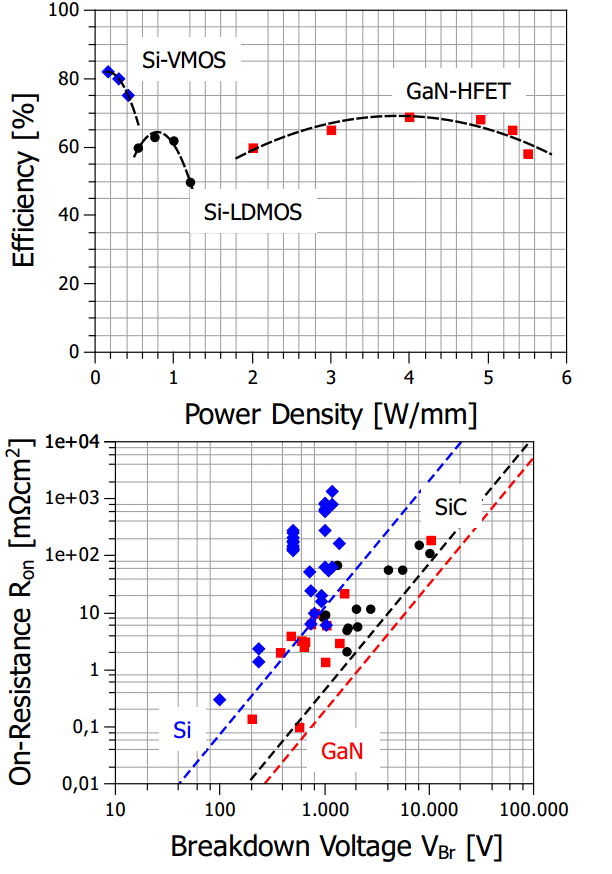
\includegraphics[width=0.4\textwidth]{TransistorPerf}
\caption{Comparative performance of power switch types, Reproduced from\cite{Krausse2013}}
\label{GaNCharacter}
\end{figure}
\indent To conclude discussion on power switches, the literature proposed novel circuit designs to improve switching efficiency. The limitations of these designs focus attention on the switch devices. The literature indicates as voltage and power density demands of a design increase, non-standard CMOS process and CMOS alternatives become increasingly attractive.\\
\textbf{Capacitors: }After Viraj et al.\cite{Viraj2007}, much research effort was expended regarding converter capacitor energy density and impedance modulation. Kwong et al.\cite{Kwong2009} address both issues uniquely. The load is a sub-threshold processor, which allows low-energy density capacitors to provide adequate drive. Converter impedence is reduced with technology options and circuit topology. Metal insulator metal (MIM) capacitors are used as power passives. MIM capacitors have the desirable qualities of being compatible with bulk CMOS and having a high $Q_c$. Their disadvantage is low energy density. Viraj et al.\cite{Viraj2007} observed an exponential deterioration of efficiency with mismatched load impedance. This work implements a re-configurable step-down voltage circuit, where output capacitors can be stacked for 4 step-down voltages or 4 converter impedances.\\
Kwong et al. stands alone in the literature because it uses a sub-vt processor load to mitigate low energy density where most literature attempts to improve it.\\
\indent Le et al. \cite{Phuck2010} propose a novel converter circuit topology with more granular impedance modulation control. By splitting $C$ into 4 parallel SC converter modules, $Z_O$ is adjusted by modulating the phase difference between the $F_s$ of these modules. The converter also features the re-configurable step-down voltage circuit for coarse grain voltage control. Peak efficiency is far higher than \cite{Viraj2007} at 82\%, and the efficiency curve has linear regions as opposed to the purely exponential worsening of \cite{Viraj2007}.\\
\indent Regarding energy density, non-standard CMOS capacitors dominate contemporary integrated converter literature.\\
Since energy density is improved by reducing loss, early work explored the limit of CMOS with circuit techniques. Besides their other innovations, Kwong et al.\cite{Kwong2009} feature a charge recycling circuit. The operating principle is similar to \cite{Alimadadi2008}, but the energy source is parasitic capacitance and bondwire inductance. The technique was not implemented in later designs by the authors or others.
\indent Later work focuses on technology options for improving energy density. In CMOS compatible technologies, MIM~\cite{Kwong2009} and Thin-gateMOS/fringe metal~\cite{Pique2012} capacitors are succeded by the exotic Deep trench~\cite{Pique} and Ferroelectric~\cite{Damak2013} capacitors.\\
Exotic capacitor types either greatly increase $C$ per unit area because they realise an extremely high permittivity ($\epsilon_r$). Capacitance may be calculated $C = \epsilon_r \times \frac{A_p}{l_p}$ where $A_p$ is the area of capacitive plates and $l_p$ is the separation distance. 
\begin{table}
    \begin{tabular}{|l|l|l|}
    \hline
    Capacitor               & Material & Permittivity ($\epsilon_r$) \\ \hline
    Bulk CMOS~\cite{Robertson2004}               & SiO2     & 3.9          \\ \hline
    High K CMOS~\cite{Robertson2004}             & HfSiO4   & 11           \\ \hline
    *Deep trench (structure)~\cite{Johari2009} & PZT      & 1000         \\ \hline
    *Ferroelectric~\cite{Lee2004}			& BaTiO3      & $\approx$4600         \\ \hline    
    \end{tabular}
\end{table}
\textit{* example technologies, not used in reviewed designs}
High $\epsilon_r$ can effectively negate bottom and top plate parasitic capacitance, since these capacitors could have an $\epsilon_r$ several orders of magnitude lower than the power capacitors.\\ 
To close on the topic of high $\epsilon_r$, Deep trench and Ferroelectric capacitors designs do not exhibit multiple order of magnitude power density improvements over others. In these technologies, $\epsilon_r$ varies with greatly with temperature \cite{Lee2004} and frequency \textbf{Get paper ref}. %http://www.mrl.ucsb.edu/~seshadri/old/MATRL100A/class13.pdf
Further research is needed to understand their limits in power converters.\\
Another class of converters has gained prominence due to the difficulties of energy density in capacitors. Semi-integrated converters \textbf{Cite a bunch} use off-die capacitors as a charge source. Provided such capacitors can be connected to the rest of a converter with a very low inductive path, these designs offer higher drive capability at the cost of an extra component.\\
\indent In summary of capacitors, early circuit level approaches to energy density have been superceded by non-standard CMOS. Architectural level approaches in SC designs have been successful in improving impedance modulation.

\indent To summarise power component literature, power switches offer many options for design trade-off. Passive components were limited in energy density with standard CMOS. Recent advances in device physics have succeeded in miniturising energy dense inductors and capacitors, but these require additional doping material and process steps to create on bulk Si.\\



%\textbf{System: well defined, class of problems: well defined, now we will see "fixed" systems}\\
\begin{itemize}
%\item{Switches fixes paper list and description DONT USE EXOTIC TECH! THESE WERE NEVER USED ON INTEGRATED DESIGNS!!!}
\item{Control fixes paper list and description NOTE THAT THIS PROBLEM IS WELL UNDER CONTROL, CONCLUDE FROM THIS SECTION} Le note that splitting $C$ into parallel converter modules improves the terrible ripple of SC converters, 41phase of Pique takes this to the next level. all those phases greatly smooth ripple but this is an architecture/control technique
%\item{Capacitor fixes paper list and description NOTE THAT THIS PROBLEM CANNOT BE "SOLVED" FROM A SC TOPOLOGY POINT OF VIEW AND INDUCTORS ARE "BETTER" IN TERMS OF ENERGY DENSITY AND LINE REGULATION. Note faliures: MIT charge recycling work did not work!. Figured out loss conditions capacitors here: A 32nm Fully Integrated Reconfigurable Switched-Capacitor DC-DC Converter Tried to mitigate bottom plate parasitics with fractal caps.defined here:\cite{Samavati2008} but not the paper }
\item{Inductor fixes paper list and description. NOTE THAT THIS IS "SOLVED" BUT FOR SEMI-INTEGRATED OR WHATEVER note topology fixes, flying capacitor is used}
We note that the approach is not necesarily to increase the size of inductance, but the quality factor. the baseline CMOS \cite{Alimadadi2008} realized 4.38nH inductors which is comprable with \textbf{HKGuys} at \textbf{5.xnH}, but the later work is able to realize a far greater energy density due to the novel technique of using bondwire as inductors.
%\item{SC Ripple Fixes} % Fully Integrated Capacitive DC-DC Converter wit all digital Ripple Mitigation technique
\end{itemize}

\section{Saving pins with DC DC converters}

\textbf{Solutions \& Stakeholders, why is there still work to be done?}\\
Need to define the problem of Signal to power pin ratio. We cannot optimize this today with DC DC converters, because the \@ CMOS voltage stepdown means we need to have a lot of CORE power pins.\\
Our "stakeholder" is high voltage stepdown. If we do it we could reduce \textbf{DEFINE}"CORE POWER PINS" to an amount desirable for \textbf{DEFINE} signal integrity\\
Now we can outline the high voltage work that was summarized in the google doc I did

\subsection{The IO limit with integrated DC DC converters}

\textbf{Defines stakeholder specific problem}\\
Think about this, it has to be differentiated from the section above

\subsection{Solutions}

Here we have to talk about:\\
3 the micro transformer solution to this problem (it could be made promising) \\
2 the MIT solution to this problem (it does not look promising)\\
1 the disruptive technology of Si on Insulator, and how it could be paired with interposers\\
In the mobile segment Silicon interposers can be used to solve the IO problem as seen in [Ultra-high I/O Density Glass/Silicon Interposer for high Band-witdh Smart Mobile Application].\\
This interposer allows signal integrity to be maintained at low voltage from the interposer to memory. a High voltage from the substrate and DC DC converter integrated to the interposer allows power density to be met with fewer pins on the package. In this scenario, the package can be made smaller to allow denser integration, or the io bandwidth  can be bound to signal integrity requirements...\\


\textbf{SHOULD HAVE SOME SIMULATION TO CHECK INSIGHT ON 1, 2 and 3}\\

\subsection{Conclusions}

Basically conclude that given the solutions simulation we could reach a situation where IO pressure is lifted from core power perspective, but that isn't so great tbh. 
\textbf{Remeber Q = CV A high voltage power grid will require higher board capacitors and you need to be sure that inductance is sufficiently low on pcb as not to impede this current path}  


{\footnotesize \bibliographystyle{acm}
\bibliography{sample.bib}}


\theendnotes

\end{document}







